\subsection{Woody Fibers Decomposition Model}
Fungi with the ability to decompose lignin or cellulose~\cite{lignin}\cite{cellulose} are distributed on an ideal cylindrical dead wood. Under certain environmental temperature and moisture conditions, the hyphae begin to expand and grow, and fungi secrete biologically active enzymes that can decompose the woody fibers. As time goes by, the outer layer of woody fibers decompose and fall off, and the fungi gradually approach the axis of the dead wood. Ignoring the surface area of cylinder bottoms, use the \textit{cylinder side surface area formula}, and mark it as \textit{Eq.~(\ref{cylindersurfacearea})}
\begin{equation}
  \label{cylindersurfacearea}
  S_{cylinder} = 2\pi r\cdot h
\end{equation}
where $r$ represents the radius of dead wood, and $h$ represents the total length of dead wood. As the radius decreases, it comes to a conclusion that the surface area of cylinder also decreases.
\par
Based on the conclusion, it is obvious that the number of fungi per unit area would increase. Meanwhile, fungal hyphae can generally grow to several times their initial size~\cite{initialsize}. Therefore, even considering the loss of fungi because of wind and rain, the number of fungi would still increase significantly as their distribution gradually approaches the central axis.
\par
Combining with the relevant knowledge of electromagnetic in physics~\cite{physics}, we find that the distribution of fungi has many similarities with the \textit{Gaussian surface} in the electric field. On the one hand, the distribution of fungi is cylindrical and could be represented by a cylindrical Gaussian surface. On the other hand, as the radius decreases, both the electric field strength and the number of fungi per unit area (also known as fungi decomposition rate) would increase. From \textit{Gauss theorem}, the decomposition cylinder is shown in \textit{Figure~1}, and  we can get \textit{Eq.~(\ref{secondeq})}, \textit{Eq.~(\ref{thirdeq})} and \textit{Eq.~(\ref{fourtheq})} as follows.
\begin{figure}[H]
  \centering
  \label{figure1}
  \subfigure[Electric field intensity $\bm{E}$ and area differential $d\bm{S}$.]{
    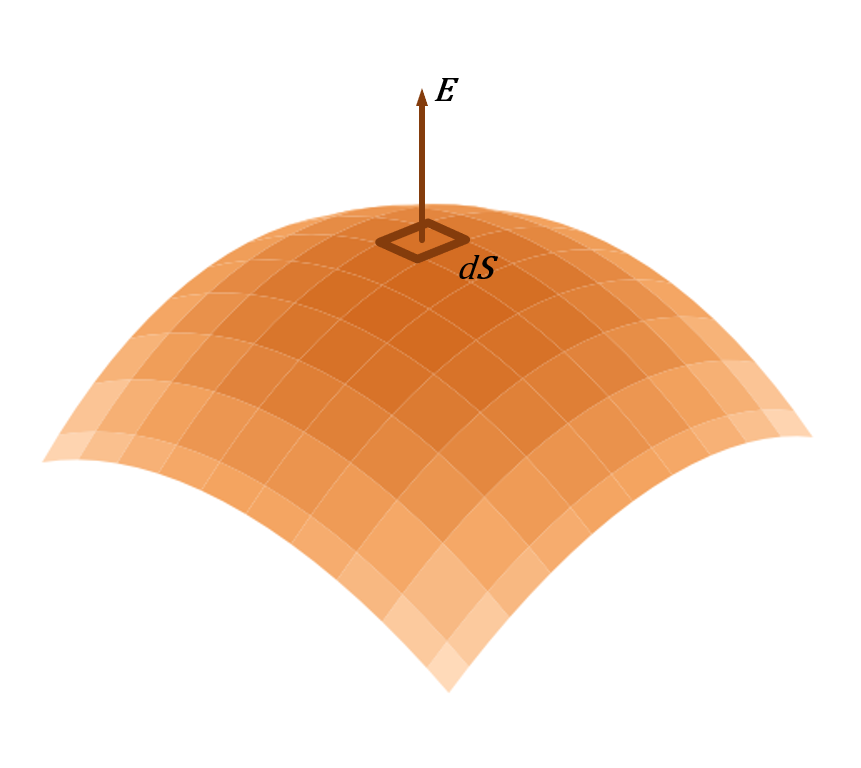
\includegraphics[width=0.45\textwidth]{figures/plain.png}
  }
  \subfigure[Ideal cylindrical wood.]{
    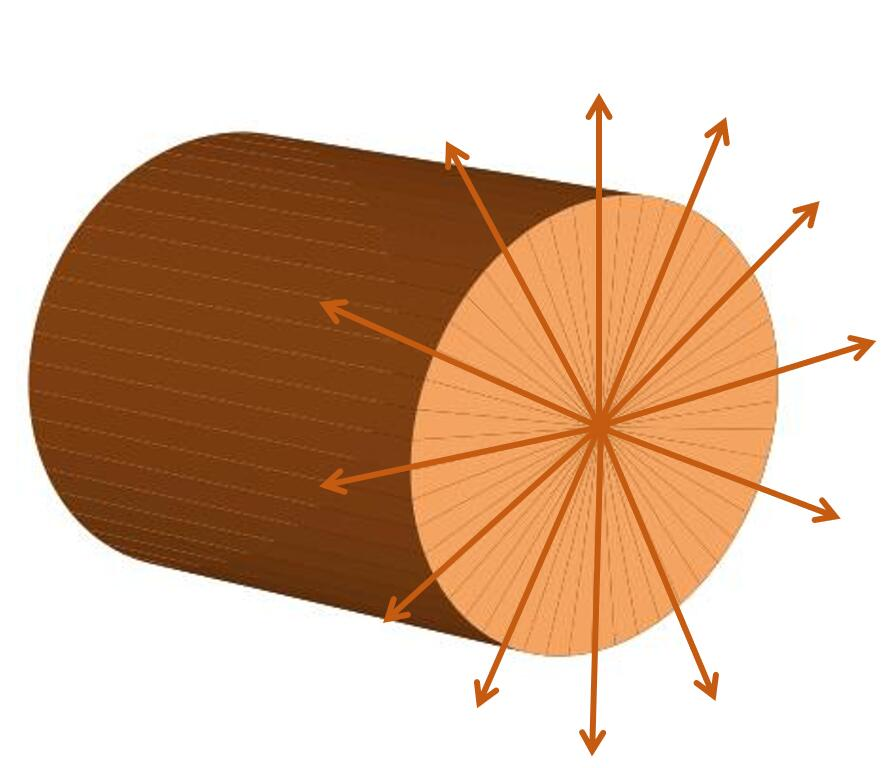
\includegraphics[width=0.45\textwidth]{figures/cylinder.jpg}
  }
  \caption{Decomposition cylinder.}
\end{figure}
\begin{equation}
  \label{secondeq}
  \oint_S \bm{E} \cdot d\bm{S}=\frac{1}{\varepsilon}\int_V \rho d V
\end{equation}
\begin{equation}
  \label{thirdeq}
  \bm{E}=\frac{\lambda}{2\pi \varepsilon R}
\end{equation}
\begin{equation}
  \label{fourtheq}
  \Phi = \oint_S \bm{E}\cdot d\bm{S} = \oint_S \frac{\lambda}{2\pi\varepsilon R}d S = \frac{\lambda}{2\pi\varepsilon R} 2\pi R l = \frac{\lambda l}{\varepsilon}
\end{equation}
where $\bm{E}$ represents electric field intensity on the surface of a uniformly charged cylinder, whose direction is radial, and $\Phi$ represents electric flux. Convert the above electromagnetic equations and parameters into formulas for estimating the decomposition rate ($\bm{DR}$) of fungi in \textit{Eq.~(\ref{fiftheq})}, \textit{Eq.~(\ref{sixtheq})} and \textit{Eq.~(\ref{seventheq})}
\begin{equation}
  \label{fiftheq}
  \oint_S DR\cdot dS = \frac{1}{\varepsilon_{DR}}\sum N_{inside} = \frac{1}{\varepsilon_{DR}} \int_V \rho dV
\end{equation}
\begin{equation}
  \label{sixtheq}
  DR = \frac{\alpha}{2\pi \varepsilon_{DR} R}
\end{equation}
\begin{equation}
  \label{seventheq}
  ACT=\oint_S DR\cdot dS = \oint_S \frac{\alpha}{2\pi \varepsilon_{DR} R} dS = \frac{\alpha}{2\pi \varepsilon_{DR} R} 2\pi R h = \frac{\alpha h}{\varepsilon_{DR}}
\end{equation}
where $\alpha$ represents fungi linear density, $DR$ represents the decomposition rate, $\varepsilon_{DR}$ represents environmental decomposition constant determined by surrounding meteorological indicators, and $ACT$ represents the \textbf{fungal activity factor}, which is determined by the suitable living concentration of specific fungal types, moisture tolerance and the influence between different fungal species. According to \textit{Eq.~(\ref{sixtheq})}, as fungi gradually approach the central axis, the decomposition rate of fungi increases, which is consistent with the previous analysis.